\chapter{Usando \maggen}
\label{chap:usos}
\minitoc
Para usar \maggen\ debemos invocar la herramienta mediante la linea de comando, es decir, debemos contar con una terminal\footnote{En sistemas \textit{windows} compatible: win+R y luego \texttt{cmd} y en sistemas \textit{unix}: Alt+f2 y luego \texttt{xterm}} para su funcionamiento. Por cuestiones de simpicidad y flexibilidad de la herramienta, no se considero el desarrollo de un \textit{front-end} para \maggen. Además, debemos tener en cuenta, que el usuario presentara interes en el resultado generado de \maggen y no de una innecesaria interfaz grafica, que entorpeceria su comportamiento conbinatorio con otros comandos.
  
\maggen\ puede ser invocado utilizando una serie de parametros que inciden directamente sobre el resultados producido por la herramienta. En el desarrollo de este capitulo trataremos estos temas en detalles y ademas analizaremos el uso del evaluador generado por \maggen.

\section{Uso de \maggen: Parametros y opciones}
La totalidad de parametros y opciones de \maggen\ son opcionales. La sintaxis de invocacion de la herramienta esta dada por:\\
\begin{center}\texttt{maggen [OPTIONS]}\end{center}
Las opciones son las siguientes:
\begin{description}
\item [-f  file] Definir el archivo de entrada de \maggen como \texttt{file}.
\item [-i  header] Incluir \texttt{header} en la generacion de codigo. Genera un \texttt{\#include ``header''} del archivo que referencia esa ruta. Dicha linea, \maggen la agrega al archivo generado.
\item [-fo folder] Define \texttt{folder} como el directorio de salida para \maggen.
\item [-o  name] Define a \texttt{name} como el nombre de la clase y del archivo generado por \maggen.
\item [-h] Muestra mensaje de ayuda.
\end{description}

Si invocamos:\\\texttt{maggen -h} obtenemos el siguiente mensaje de ayuda:
\begin{center}
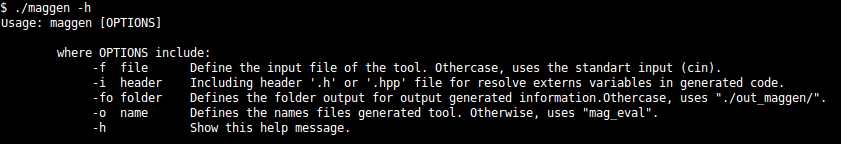
\includegraphics[width=350pt,height=60pt]{help.png}
\end{center}
 

\section{Uso del evaluador generado}
bla bla